%!TEX program = xelatex

% 完整编译: xelatex -> bibtex -> xelatex -> xelatex
\documentclass[lang=cn,11pt,a4paper]{elegantpaper}

% 这个模板有一点点的问题,其引用好像不太形

\title{Learning with Sparsity}
\author{Zhenwei Lin }
% \institute{\href{https://elegantlatex.org/}{Elegant\LaTeX{} 项目组}}

% \version{0.08}
\date{\zhtoday}

\theoremstyle{plain}
\newtheorem{thm}{Theorem}[section]
\newtheorem{lem}{Lemma}[section]
\newtheorem{prop}{Proposition}[section]
% \newtheorem*{cor}{Corollary}[section]

% \theoremstyle{definition}[section]
\newtheorem{defn}{Definition}[section]
\newtheorem{conj}{Conjecture}[section]
\newtheorem{exmp}{Example}[section]

\theoremstyle{remark}
\newtheorem*{rem}{Remark}



\usepackage{appendix}
\usepackage{varioref}
\usepackage[ruled,vlined]{algorithm2e}
\renewcommand{\appendixtocname}{附录}
\renewcommand{\appendixpagename}{附录}
\begin{document}

\maketitle

\begin{abstract}
% 本文为 \href{https://github.com/ElegantLaTeX/ElegantPaper/}{ElegantPaper} 的说明文档。此模板基于 \LaTeX{} 的 article 类,专为工作论文写作而设计。设计这个模板的初衷是让作者不用关心工作论文的格式,专心写作,从而有更加舒心的写作体验。如果你有其他问题、建议或者报告 bug,可以在 \href{https://github.com/ElegantLaTeX/ElegantPaper/issues}{Github::ElegantPaper/issues} 留言。如果你想了解更多 Elegant\LaTeX{} 项目组设计的模板,请访问 \href{https://github.com/ElegantLaTeX/}{Github::ElegantLaTeX}。
本文主要为从优化角度来对监督学习进行介绍
\keywords{loss function; penalty function}
\end{abstract}

\section{Loss function}

\subsection{linear regression}
\begin{equation}\nonumber
    \begin{aligned}
        l(y,f(x)) =& (y-f(x))^2\\
        H(f) =& \left\{ f|f(x) = a^Tx+b \right\}\\
        \Rightarrow \min _{l} =& \min \frac{1}{N} \sum_{i=1}^{N}(y_i-a_i^Tx_i-b)^2
    \end{aligned}
\end{equation}

\subsection{LAD regression}
\begin{equation*}
    l(y,f(x)) = \left| y-f(x) \right| 
\end{equation*}
\subsection{0-1 loss-function}
\begin{equation*}
    l(y,f(x)) = \left\{\begin{array}{l}
        1\quad y=f(x)\\
        0\quad y \ne f(x)
    \end{array}\right.
\end{equation*}

\subsection{sign function}
\begin{equation*}
    \begin{aligned}
        f:X&\rightarrow Y \subseteq R\\
        G(x) =& Sign(f(x))\\
        l(y,G(x)) =& \left\{\begin{array}{l}
         1\quad y\cdot f(x) <0\\
         0\quad y\cdot f(x) \geq 0  
        \end{array}\right.
    \end{aligned}
\end{equation*}
\begin{center}
    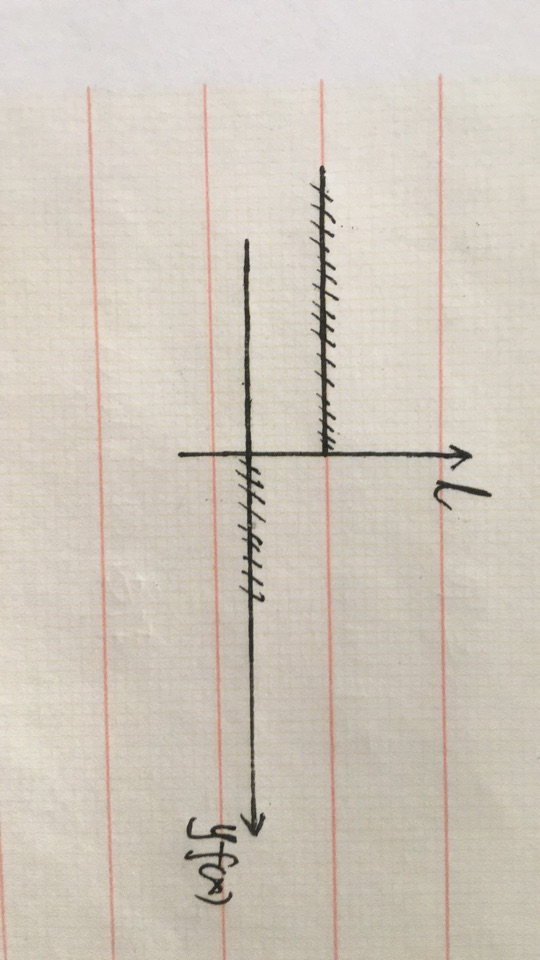
\includegraphics[width = 8cm,angle = 90]{fig/loss.png}
\end{center}
为了逼近上面这个函数曲线,我们在不同模型中选取了不同的函数来逼近,具体的有logistic regression, Adaboost,SVM.

\subsection{logistic regression}
\begin{equation*}
    l(y,f(x)) = log(1+exp(yf(x)))
\end{equation*}
\subsection{Adaboost}
$$ l(y,f(x)) = exp(yf(x)) $$
\subsection{SVM}
$$ l(y,f(x)) = (1+yf(x))_{+} $$

\section{logistic regression}
\begin{equation}
    \begin{aligned}
        D =& \left\{ (x_i,y_i) \right\}_{i=1}^N,y_i \in \left\{ -1,1 \right\}  \\
        p(Y_i= 1) &= \frac{exp(x"_i^T\beta)}{1+exp(x_i^T\beta)} = \frac{1}{1+exp(-x_i^T\beta)}\\
        p(Y_i=-1) &= \frac{1}{1+exp(x_i^T\beta)}\\
        p(Y_i) &= \frac{1}{1+exp(-y_ix_i^T\beta)}\\
        \Rightarrow& \min _{\beta} \sum_{i=1}^{N} log(1+exp(-y_ix_i^T\beta)) 
    \end{aligned}
\end{equation}

如何解这个最小化问题呢?

\begin{equation*}
    \begin{aligned}
        f(z) = &log(1+exp(-z))\\
        f^{\prime}(z) =& -\frac{exp(-z)}{1+exp(-z)}\\
        f^{\prime\prime}(z) =& f(z)(1-f(z)) \leq \frac{1}{4}\\
        \nabla {l(\beta)} =& -\sum_{i=1}^{N}\frac{exp(y_ix_i^T\beta)}{1+exp(y_ix_i^T\beta)}\cdot y_ix_i = X^Tdiag(Y)P \quad
        P = \left[\begin{array}{c}
            \frac{exp(-y_1x_1^T\beta)}{1+exp(-y_1x_1^T\beta)}\\\vdots 
        \end{array}\right]\\
        \nabla ^2{l(\beta)} =& \sum_{i=1}^{N}\frac{exp(y_ix_i^T\beta)}{1+exp(y_ix_i^T\beta)}y_i^2x_ix_i^T = X^Tdiag(P(1-P))X \leq \frac{1}{4}\lambda _max(X^TX)
    \end{aligned}
\end{equation*}
因此可以采用 $\frac{1}{\beta} = \frac{4}{\lambda_{max}(X^TX)}$ 的step来对其进行下降 

\subsection{newton's method}
\begin{equation*}
    \begin{aligned}
    \beta_{t+1} =& \beta_t + (\nabla^2{l(\beta_t)})^{-1}\nabla {l(\beta_t)} \\
    =&\beta _t + (X^TwX)^{-1}X^Tdiag(Y)P\quad denote w = diag(P(1-P))\\
     &\begin{array}{c}
        = (X^TwX)^{-1} X^Tw\underbrace{(X\beta_t+X^Tdiag(Y)P)}\\z_t
    \end{array}
    \end{aligned}
\end{equation*}

这个其实对应的是加权最小二乘的解 $argmin_{\beta} \left\{ (z_t-X\beta)^Tw(z_t-X\beta) \right\}  $ 

若其中同样存在不可逆的问题,则选择sparse logistic regression 的方法来建模
$$ \min_{\beta} \left\{ \frac{1}{2N} \sum_{i=1}^{N}log(1+exp(-y_ix_i^T\beta))+\lambda_N \left\| \beta \right\|_1  \right\}  $$

\section{AdaBoost}
Q:Can we construct a strong classifier based on existed weak classifiers?

\begin{algorithm}[H]
    \SetAlgoLined
     Input $\left\{ (x_i,y_i) \right\}_{i=1}^N,y_i \in \left\{ -1,1 \right\} ,m=1 $,sample weight $w_i = \frac{1}{N}$  \;
     \While{$m \leq M$ }{
      step1:Fit a classifier $G_m(x)$ based on train set D 
      $$ G_m(x) = argmin \sum_{i=1}^N I(y_i\ne G_m(x_i))\cdot w_i^m $$
     
     step2: 计算错分率
     $$ err_m = \frac{\sum_{i=1}^Nw_i^mI(y_i \ne G_m(x_i))}{\sum w_i^m} $$
     
     step3:更新权重,分对权重不变,分错权重增加
     $$ w_i^{m+1} \leftarrow w_i^m exp(\alpha_m\cdot I(y_i \ne G_m(x_i))) $$
     $$ \alpha_m = log(\frac{1-err_m}{err_m}) $$
     $$ m \leftarrow m+1 $$
     step4:renormalization $$ \sum w_i^{m+1} = 1 $$
     }
     Output: Majority Volting
     $$ G(x) = Sign \left[\sum_{m=1}^M\alpha_m G_m(x)\right] $$ 总共有M个弱分类器
     \caption{AdaBoost}
    \end{algorithm}

% \begin{algorithm}[H]
%     \SetAlgoLined
%     \KwResult{Write here the result }
%      initialization\;
%      \While{While condition}{
%       instructions\;
%       \eIf{condition}{
%        instructions1\;
%        instructions2\;
%        }{
%        instructions3\;
%       }
%      }
%      \caption{How to write algorithms}
%     \end{algorithm}

 算法2,之后我们再说明二者是等价的。

\begin{algorithm}[H]
    \SetAlgoLined
     Input $\left\{ (x_i,y_i) \right\}_{i=1}^N,y_i \in \left\{ -1,1 \right\},f^{(0)}(x_i)=0,m =1$\;
     \While{$m \leq M$ }{
      step1:Compute $$ (\hat{\beta}_m,G_m(x)) = argmin\sum l ( y_{i},f^{(m)}(x_i)+\beta_mG_m(x) )  $$
     
     step2: $$f^{(m+1)}(x) = f^{(m)}(x)+\hat{\beta}_m G_m(x)$$
     $$ m\leftarrow m+1 $$
     }
     Output: 
     $$ G(x) = Sign (f^{(M)}(x)) = Sign\left\{ \sum_{m=1}^M \hat{\beta}_m G_m(x) \right\}  $$ 
     \caption{Forward Stepwise Additive Model}
    \end{algorithm}

\newpage
\begin{theorem}
    AdaBoost is equivalent to the forward Stepwise Additive Model by using the exponential error $l(z) = exp(-z)$ 
\end{theorem}

\begin{proof}
    \begin{equation*}
        \begin{aligned}
            \sum_{i=1}^N l(y_i,f^{m}(x_i)+\beta_m G_m(x_i)) =& \sum_{i=1}^N exp \left\{-y_i\cdot(f^{(m)}(x_i)+\beta_mG_m(x_i))  \right\} \\
             =& \sum_{i=1}^{N} exp(-y_if^{(m)}(x_i))exp(-y_i\beta_m G_m(x_i))\\
             =& \sum_{i=1}^{N} w_i^{(m)}exp(-\beta_m y_i G_m(x_i))\\
             =&e^{\beta_m} \sum_{y_i\ne G_m(x_i)}w_i^{(m)}+e^{-\beta_m} \sum_{y_i =  G_m(x_i)}w_i^{(m)}\\
             =&e^{\beta_m} \sum_{y_i\ne G_m(x_i)}w_i^{(m)}-e^{-\beta_m} \sum_{y_i\ne G_m(x_i)}w_i^{(m)}+e^{-\beta_m} \sum w_i^{(m)}
        \end{aligned}
    \end{equation*}
$$ (e^{\beta_m}-e^{-\beta_m}) \sum w_i^m \cdot I(G_m(x_i)\ne y_i) + \sum w_i^m e^{-\beta_m} \overset{\Delta}{=}l(\beta)$$
$$ \Rightarrow G_m(x) = argmin_{G_m(x)} \sum w_i^m I(G(x_i)\ne y_i) $$
$$ \nabla{l(\beta_m)} = (e^{\beta_m}+e^{-\beta_m})\sum w_i^m I(G_m(x)\ne y_i)-e^{-\beta_m} \sum w_i^m = 0$$
$$\Rightarrow \hat{\beta}_m = \frac{1}{2} log\frac{1-err_m}{err_m} = \frac{\alpha_m}{2} $$
$$ G(x) = Sign(\sum \hat{\beta}_m G_m(x)) = Sign(\sum \frac{\alpha_m}{2}G_m(x)) $$
二者的优化问题,故二者等价
\end{proof}
















\end{document}
